\documentclass{article}

% ================================= Global settings

\usepackage{amsmath}
\usepackage{amsfonts}
\usepackage{cite}
\usepackage{hyperref}
\usepackage{tikz}
\usepackage{subcaption}
\usepackage{float}

%\usepackage[margin=2cm]{geometry}

\tikzstyle{hyperedge} = [fill,opacity=.5,fill opacity=.5,line cap=round, line join=round, line width=0pt]

% =================================================

\begin{document}

\section{Introduction}

Propositional satisfiability problem (SAT) is the problem of determining whether a propositional formula in conjunctive normal form (CNF) is satisfiable, i.e. if there exists a truth assignment of variables that satisfies the formula.
Such assignments are called models.
Propositional formulas can be thought of as finite sets of clauses, which in turn are finite sets of literals.
A literal is either a propositional variable or its negation.
Given a CNF formula, a model thus satisfies all its clauses, that is, it sets at least one literal in each clause to true.
Propositional model counting, \#SAT, is a related but harder problem of determining the amount of satisfying truth assignments of a CNF formula.

The complexity class P consists of all problems that can be solved in polynomial time; NP is a class of all problems the solutions of which can be verified in polynomial time. SAT is well known to be NP-complete.
The counting counterpart of NP is the class \#P.
\#SAT has been shown to be \#P-complete and remains \#P-hard even when syntactical restrictions on the input CNF formulas are introduced \cite{DBLP:conf/sat/GanianS17}.
However, there has been research on structural restrictions \cite{DBLP:conf/sat/GanianS17, DBLP:conf/sat/CapelliDM14, DBLP:conf/sat/GanianPSSS22, DBLP:conf/sat/SaetherTV14, DBLP:journals/dam/FischerMR08, DBLP:journals/jda/SamerS10, DBLP:journals/fuin/GanianHO13} which lead to efficient algorithms for \#SAT.

Structural restrictions are defined according to a parameter on some graph associated with the problem instance.
In case of \#SAT, such graphs often describe the relationship between the variables and/or clauses of the formula.
%Common examples include {\em primal}, {\em dual} and {\em incidence graphs}.
A certain parameter $k$, usually a positive integer, is then determined for this graphic representation of a propositional formula. 
If it's then possible to show that for some fixed $k$, there exists an algorithm that can compute \#SAT in time $f(k)n^{O(1)}$, where $f$ is a computable function and $n$ is the size of the formula, we say that \#SAT is {\em fixed-parameter tractable} when parameterized by $k$ \cite{DBLP:conf/sat/GanianS17}.
As one can see, for a fixed $k$ the term $f(k)$ is a constant, basically meaning that the runtime of the parameterized algorithm is polynomial for such $k$, and such algorithm can therefore be assumed efficient (tractable). The class of fixed parameter tractable problems is denoted FPT.
Its non-parameterized counterpart, FP, is the class of functional problems solvable in polynomial time.

This thesis is organized as follows.
In Section 2, we provide the necessary formal definitions, in particular with regards to graphical representations of formulas, and introduce several structural restrictions, among which are {\em treewidth}, {\em clique-width}, {\em disjoint branches}, {\em twin-width}, {\em rank-width}, {\em ps-width}, and others.
\textbf{[TODO: don't forget organization]}

% ---- NEW
\section{Preliminaries}

We first introduce some notions from graph theory which will be useful in this thesis.
We will use these notions to represent propositional formulas, and then perform transformations on them to obtain the desired width parameters.
For examples, see Fig. \ref{fig:graphs}.\\

\begin{figure}
	\centering
	\begin{subfigure}[b]{0.22\textwidth}
		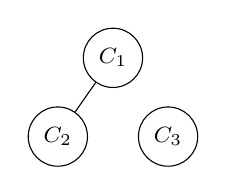
\begin{tikzpicture}[nodes=circle, nodes=draw, font=\footnotesize, minimum size=21pt]
	\node (1) at (0, 0) {$C_1$};
	\node (3) at (-0.7, -1) {$C_2$};
	\node (7) at (0.7, -1) {$C_3$};
	
	\draw (1) to (3);
\end{tikzpicture}

		\caption{}
		\label{fig:consensus}
	\end{subfigure}
	\begin{subfigure}[b]{0.38\textwidth}
		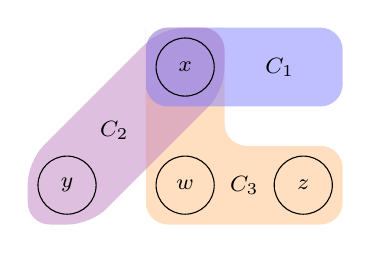
\begin{tikzpicture}[font=\footnotesize, minimum size=21pt]
	\node[circle, draw] (x) at (0, 0) {$x$};
	\node[circle, draw] (y) at (-1.5, -1.5) {$y$};
	\node[circle, draw] (w) at (0, -1.5) {$w$};
	\node[circle, draw] (z) at (1.5, -1.5) {$z$};
	
	\node (c1) at (1.2,0) {$C_1$};
	\node (c2) at (-0.9,-0.8) {$C_2$};
	\node (c3) at (0.75,-1.5) {$C_3$};
	
	\pgfdeclarelayer{background}
	\pgfsetlayers{background,main}
	
	\begin{pgfonlayer}{background}
	\begin{scope}[transparency group,opacity=0.5]
		\fill[hyperedge,color=orange,rounded corners=8pt]
		([shift=({-0.5,0.5})] x.center) -- ([shift=({-0.5,-0.5})] w.center) -- ([shift=({0.5,-0.5})]z.center) -- ([shift=({0.5,0.5})]z.center) -- ([shift=({0.5,0.5})] w.center) -- ([shift=({0.5,0.5})] x.center) -- ([shift=({-0.5,0.5})] x.center) -- ([shift=({-0.5,-0.5})] w.center);
		
		\fill[hyperedge,color=violet,rounded corners=8pt]
		([shift=({0.5,0.5})] x.center) -- ([shift=({-0.3,0.5})] x.center) -- ([shift=({-0.5,0.3})] y.center) -- ([shift=({-0.5,-0.5})] y.center) -- ([shift=({0.3,-0.5})] y.center) -- ([shift=({0.5,-0.3})] x.center) -- ([shift=({0.5,0.5})] x.center) -- ([shift=({-0.3,0.5})] x.center);
		
		\fill[hyperedge,color=blue,rounded corners=8pt]
		([shift=({-0.5,0.5})] x.center) -- ([shift=({-0.5,-0.5})] x.center) -- ([shift=({2,-0.5})] x.center) -- ([shift=({2,0.5})] x.center) -- ([shift=({-0.5,0.5})] x.center) -- ([shift=({-0.5,-0.5})] x.center);
	\end{scope}
	\end{pgfonlayer}
\end{tikzpicture}

		\caption{}
		\label{fig:hypergraph}
	\end{subfigure}
	\begin{subfigure}[b]{0.3\textwidth}
		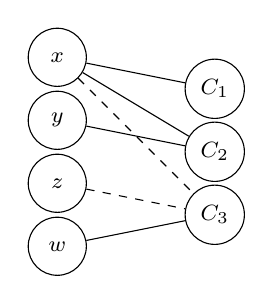
\begin{tikzpicture}[nodes=circle, nodes=draw, font=\footnotesize, minimum size=21pt]
	% consensus
	\node (x) at (0, -0.6) {$x$};
	\node (y) at (0, -1.4) {$y$};
	\node (z) at (0, -2.2) {$z$};
	\node (w) at (0, -3) {$w$};
	
	\node (c1) at (2,-1) {$C_1$};
	\node (c2) at (2,-1.8) {$C_2$};
	\node (c3) at (2,-2.6) {$C_3$};
	
	\draw (x) to (c1);
	\draw (x) to (c2);
	\draw[dashed] (x) to (c3);
	
	\draw (y) to (c2);
	
	\draw[dashed] (z) to (c3);
	\draw (w) to (c3);
\end{tikzpicture}

		\caption{}
		\label{fig:trigraph}
	\end{subfigure}
	\caption{
		Some graphical representations of the formula $C_1 \land C_2 \land C_3$ with $C_1 = \{x\}$, $C_2 = \{x,y\}$ and $C_3=\{\neg x, \neg z, w\}$.
		Here, (a) is the consensus graph, (b) the primal hypergraph, and (c) the signed incidence graph (negative edges are dashed).
		Notice how in (a), $C_3$ does not have any edges, as its literal $\neg x$ appears negated in all other clauses.
	}
	\label{fig:graphs}
\end{figure}

\noindent
\textbf{Graphs}.
A graph is a pair $G = (V,E)$ with a vertex set $V$ and an edge set $E$.
An edge $e=uv$ connects the vertex $u$ to $v$.
A graph is called {\em bipartite} if the vertices can be partitioned into two disjoint sets, and every edge has endpoints in both sets.
There are several commonly known graphs one can define for CNF formulas, such as {\em primal, dual} and {\em incidence graphs}.
In a primal graph, variables of the formula are the graph's vertices, and two vertices are connected by an edge iff both corresponding variables appear together in a clause.
A dual graph's vertices are its clauses, and two vertices are adjacent iff their corresponding clauses share a variable.
An incidence graph is a bipartite graph with variables and clauses both being vertices, and a variable is connected with a clause by an edge iff the variable appears in the clause.
A more recently studied graph is the {\em consensus graph}, where the vertices are the clauses of the formula, and two vertices are connected by an edge iff the clauses do not clash, that is, there exists no literal in one of the clauses that appears negated in the other clause.\\

\noindent
\textbf{Hypergraphs}.
A hypergraph $H=(V,E)$ with vertex set $V$ and (hyper)edge set $E$ is a generalized notion of graphs, where edges may connect not only two, but any amount of vertices.
As such, an edge is a set of vertices it connects.
A CNF formula can be represented by a primal hypergraph, whose vertices are the formula's variables, and hyperedges are the clauses, i.e. hyperedges connect the variables that appear in the clause.\\

\noindent
\textbf{Trigraphs.}
A trigraph $G=(V,E,E')$ is a graph that distinguishes two classes of edges, $E$ and $E'$.
Often such two classes are positive and negative edges, denoted $E_+$ and $E_-$, respectively, in which case the trigraph is called a {\em signed graph}.
A {\em signed trigraph} distinguishes, apart from positive and negative edges, also one more class of edges.
With a CNF formula we associate a signed bipartite incidence graph, where the two classes of vertices are the formula's clauses and variables, and an edge connects a variable with the clause where it appears, with the appropriate sign (according to whether the variable occurs positively or negatively in the clause).

\subsection{Width Parameters}

We now proceed with an introduction of many parameters used to describe the structure of graphs, the so-called {\em width parameters}. \\

\noindent
\textbf{Treewidth} \cite{DBLP:conf/sat/GanianS17}.
For a simple, undirected, finite graph $G = (V,E)$ we define a {\em tree decomposition} to be a pair $(T, B)$, where $T$ is a tree, $B$ a set of {\em bags}, and the vertices of $T$ are the bags.
Each bag is a set of the graph's vertices.
Moreover, a tree decomposition has to fulfil the following two conditions:
\begin{enumerate}
	\item for any edge $uv\in E$ there exists some bag $B' \in B$ such that $\{u,v\} \subseteq B'$, and
	\item for any vertex $v\in V$, $T[\{ b \in B \; | \; v \in b \}]$ is a connected tree with at least one node.
\end{enumerate}
Informally speaking, tree decompositions are a structured way to ``break down'' a graph into its parts.
We define the {\em width} of a tree decomposition to be its maximum bag size minus one, and the {\em treewidth} of $G$, $\textbf{tw}(G)$, to be the minimum width over all its tree decompositions.\\

\noindent 
\textbf{Disjoint branches} \cite{DBLP:conf/sat/CapelliDM14}.
A join tree of a hypergraph $H=(V,E)$ is a pair $(\mathcal{T}, \lambda)$, where $\mathcal{T}=(N,T)$ is a tree with node set $N$ and edge set $T$, and $\lambda : N \rightarrow E$ is a bijection from tree's nodes to hypergraph's edges, which fulfils the following:
\begin{enumerate}
	\item for every $e\in E$, there exists a $t\in T$ such that $\lambda(t)=e$, and
	\item for every $v\in V$, $\mathcal{T}[\{ n \in N \; | \; v \in \lambda(n) \}]$ is a connected subtree of $\mathcal{T}$.
\end{enumerate}
Notice how the definition is similar to that of tree decompositions.
A join tree where for every two nodes $n, n'$ on different branches, $\lambda(n) \cap \lambda(n') = \emptyset$, is called a {\em disjoint branches decomposition}. 
Such decompositions represent a way to ``break down'' a hypergraph into disjoint parts (recall that $\lambda(n)$ is a hypergraph's edge).

We now consider acyclicity of hypergraphs.
In contrast to graphs, there is not just one single but several notions of acyclicity for hypergraphs, such as $\alpha$- (most general), $\beta$- and $\gamma$-acyclicity (least general), all of which can be defined using join trees.

A hypergraph is said to be $\alpha$-acyclic if it has a join tree.
One shortcoming of this definition is that a subhypergraph of an $\alpha$-acyclic hypergraph is not necessarily $\alpha$-acyclic itself.
Thus, a more restrictive notion of $\beta$-acyclicity was introduced, which requires that a hypergraph and all its subhypergraphs be $\alpha$-acyclic.
Admitting a disjoint branches decomposition is itself another notion of hypergraph acyclicity, which lies strictly between $\beta$- and $\gamma$-acyclicity.
As such, having a disjoint branches decomposition implies $\beta$- and $\alpha$-acyclicity.
Finally, a hypergraph is $\gamma$-acyclic if it admits a disjoint branches decomposition for any choice of hyperedge as the root.

Using the four introduced notions of acyclicity, we define the respective classes of hypergraphs, i.e. $\alpha$-, $\beta$-, $\gamma$-acyclic hypergraphs, as well as hypergraphs that admit a disjoint branches decomposition. \\

\noindent
\textbf{Twin-width} \cite{DBLP:conf/sat/GanianPSSS22}.
Consider a trigraph $G=(V,E,R)$ that distinguishes between black ($E$) and red ($R$) edges.
A trigraph whose subgraph induced by the red edges, that is $G[R]$, has maximum degree at most $d$, is called a {\em d-trigraph}.

A {\em contraction} of a trigraph $G$ is a trigraph $G'=G/u,v$ that is a result of contracting two vertices $u,v \in V(G)$ into a single vertex $w$, where the edges of $w$ are determined according to the following:
\begin{itemize}
	\item $wx \in E(G')$ iff $ux, vx \in E(G)$,
	\item $wx \not\in E(G') \cup R(G')$ iff $ux, vx \not\in E(G)\cup R(G),$
	\item $wx \in R(G')$ otherwise.
\end{itemize}
Intuitively, red edges represent ``errors'' that occur during a contraction.
A contraction of a $d$-trigraph is called {\em d-contraction} if it is a $d$-trigraph itself.
If there exists a sequence of $d$-contractions such that a graph is contracted into a single vertex, the graph is called {\em d-collapsible}.
The {\em twin-width} $\textbf{tww}(G)$ of a trigraph $G$ is then the minimal $d$ for which it is $d$-collapsible.

For bipartite trigraphs it is helpful to restrict contraction sequences to those where only vertices from the same partition are contracted.
That is, for a bipartite trigraph $G$ with $V(G) = A \cup B$, $A \cap B = \emptyset$, there is no contraction of the form $G/a,b$ in the sequence, where $a\in A, b\in B$.
Such sequences are called {\em bipartite contraction sequences}.
Notice that no bipartite contraction sequence can end in a single-vertex graph and therefore $d$-collapsibility does not apply.

We introduce another definition.
Say a bipartite trigraph $G$ is {\em bipartitely $d$-collapsible} if there exists a sequence of bipartite $d$-contractions such that $G$ is collapsed into a graph with two vertices.
Then, the {\em signed twin-width} $\textbf{stww}(G)$ of a bipartite trigraph $G$ is the minimal $d$ for which it is bipartitely $d$-collapsible.
In other words, it is the minimal red degree of all bipartite contraction sequences of $G$.\\

\noindent
\textbf{Clique-width} \cite{DBLP:journals/dam/FischerMR08}.
Colored graphs are graphs with vertices annotated by an integer (color) in $\{1,...,k\}$.
Consider the following set of operations on colored graphs:
\begin{enumerate}
	\item Disjoint union $\oplus$, where $V(A \oplus B)=\{ (v,\, \lambda(v)) \; | \; v \in V(A) \text{ or } v\in V(B) \}$, and $\lambda(v)=$ ``$A$'' if $v\in A$, and $\lambda(v)=$ ``$B$'' if $v\in B$,
	\item Recoloring $\rho_{i,j}(I)$, resulting in a graph where vertices colored $i$ are re-colored $j$,
	\item Edge creation:
	\begin{enumerate}
		\item for unsigned graphs, $\mu_{i,j}(I)$ results in a graph where all vertices colored $i$ are adjacent to all vertices colored $j$,
		\item for signed graphs, $\mu_{i,j}^+(I)$ or $\mu_{i,j}^-(I)$ result in a graph where all vertices colored $i$ are connected to all vertices colored $j$ by a positive or negative edge, respectively. In case of bipartite graphs, vertices from different vertex partitions are not connected.
	\end{enumerate}
\end{enumerate}

\noindent
Notice that the disjoint union is used to introduce single-vertex graphs and avoid name conflicts between vertices.
As an example, consider how one can create cliques using two colors: beginning with two single-vertex graphs $A, B$ colored, say, red (1) and blue (2) respectively, a 2-clique can be obtained as $\mu_{1,2}(A \oplus B)$, a 3-clique as $\mu_{1,2}(\rho_{2,1}(\mu_{1,2}(A \oplus B)) \oplus B)$, and so on.

{\em Clique-width} $\textbf{cw}(G)$ is defined as the minimal $k$ such that $G$ can be obtained from colored single-vertex graphs using the operations above.
From the example above it is easy to see that cliques have clique-width at most 2.\\

\noindent
\textbf{Branch-width} \cite{DBLP:journals/jct/OumS06}.
Branch-width is defined via set functions.
A set function $f$ maps a subset to a number, i.e. $f : 2^V \rightarrow \mathbb{Z}$, where $V$ is a finite set.
If for all $X,Y \subseteq V$ it holds that $f(X)+f(Y) \geq f(X\cap Y) + f(X\cup Y)$, $f$ is called {\em submodular}.
Moreover, if for all $X\subseteq V$, $f(X) = f(V \setminus X)$, $f$ is said to be {\em symmetric}.

A {\em branch decomposition} of a symmetric, submodular function $f$ is a pair $(T, \lambda)$, where $T$ is a subcubic tree (i.e., every vertex is incident with at most three edges), and $\lambda$ a bijective function from $V$ to the leaves of $T$.
If $\lambda$ is surjective, the branch decomposition is said to be {\em partial}.

For a (partial) branch decomposition $\mathcal{T} = (T,\lambda)$ of $f$ and some edge $e$, $T \setminus e$ is a forest that consists of two connected subtrees of $T$.
Thus $e$ defines a partition $(X,Y)$ of the leaves of the branch decomposition.
The width of the edge $e$ is defined as $f(\lambda^{-1}(X)) = f(\lambda^{-1}(Y))$, and the width of a branch decomposition as the maximum width of all edges of $T$.
Then, the {\em branch width} $\mathbf{bw}(f)$ of a symmetric, submodular function $f$ is the minimum width over all its branch decompositions.\\

\noindent
\textbf{Rank-width} \cite{DBLP:journals/fuin/GanianHO13}.
The definition of rank-width utilizes concepts used in the definition of branch-width.
Consider a simple graph $G$, subsets $X,Y \subseteq V(G)$ and let $\mathbf{A}_G[X,Y]$ be a binary matrix.
The entry $a_{x,y}$ of $\mathbf{A}_G[X,Y]$ is 1 iff $xy \in E(G)$, where $x\in X, y\in Y$.

A {\em cut-rank function} is a symmetric, submodular function $\rho_G : 2^{V(G)} \rightarrow \mathbb{Z}$ such that $\rho_G(X)=\rho_G(V(G)\setminus X) = \text{rank}(\mathbf{A}_G[X, V(G)\setminus X])$.
A {\em rank decomposition} is the branch decomposition of $\rho_G$.
Then, {\em rank-width} $\textbf{rw}(G)$ is the branch-width of $\rho_G$. \\


\noindent
\textbf{ps-width} \cite{DBLP:conf/sat/SaetherTV14}.
ps-width, in contrast to most width parameters introduced above, is defined specifically for propositional formulas.
For a propositional formula $F$, let $\text{var}(F)$ denote the set of variables of $F$, and $\text{cla}(F)$ the set of its clauses.
For a set $C \subseteq \text{cla}(F)$, we say $C$ is {\em precisely satisfiable} in $F$ if there exists some assignment $\tau$ such that $\tau(c)=1$ for all $c\in C$, and $\tau(c)=0$ for all $c \in \text{cla}(F)\setminus C$.
By $\mathcal{PS}(F)$ we denote the set of all sets $C$ such that $C \subseteq \text{cla}(F)$ and $C$ is precisely satisfiable.


A {\em branch decomposition} of a formula $F$ is a pair $(T, \delta)$, where $T$ is a rooted binary tree, and $\delta$ a bijection from the leaves of $T$ to $\text{var}(F) \cup \text{cla}(F)$.
For an internal (non-leaf) node $v$ of $T$, let $\delta(v) = \{ \delta(l) \; | \; l \text{ is a leaf of subtree rooted in } v \}$.
For any node $v$ of $T$, $\delta(v)$ describes certain cuts of the propositional formula.
Let $F_v$ be then a formula induced by the clauses in cla$(F)\setminus \delta(v)$ and variables in $\delta(v)$, and $F_{\overline{v}}$ a formula induced by the clauses in $\delta(v)$ and the variables in var$(F)\setminus \delta(v)$.

{\em ps-value} ps$(\delta(v))$ of a cut $\delta(v)$ is defined as max$\{|\mathcal{PS}(F_v)|, |\mathcal{PS}(F_{\overline{v}})|\}$, and the {\em ps-width} of a branch decomposition $(T,\delta)$ as max$\{ \text{ps}(\delta(v)) \; | \; v \in V(T) \}$. 
Then, the {\em ps-width} $\mathbf{psw}(F)$ of a formula $F$ is the minimal ps-width over all its branch decompositions.\\

\begin{table}
	\centering
	\begin{tabular}{r | l}
		\textbf{structural restriction} & \textbf{complexity} \\
		\hline
		primal/dual/incidence treewidth & FPT \cite{DBLP:journals/jda/SamerS10} \\
		consensus treewidth & FPT \cite{DBLP:conf/sat/GanianS17} \\
		\hline
		$\alpha$-acyclic hypergraph & \#P \cite{DBLP:conf/sat/CapelliDM14} \\
		disjoint branches & FP \cite{DBLP:conf/sat/CapelliDM14} \\
		$\gamma$-acyclic hypergraph & FP \cite{DBLP:conf/sat/CapelliDM14} \\
		\hline
		signed incidence clique-width & FPT \cite{DBLP:journals/dam/FischerMR08} \\
		incidence clique-width & XP \cite{DBLP:conf/isaac/SlivovskyS13} \\
		\hline
		signed incidence rank-width & FPT \cite{DBLP:journals/fuin/GanianHO13} \\
		signed incidence twin-width plus $k$ & FPT \cite{DBLP:conf/sat/GanianPSSS22} \\
		ps-width & FPT \cite{DBLP:conf/sat/SaetherTV14}
	\end{tabular}
	\caption{Complexity results for width parameters on \#SAT instances}
	\label{table:complexity}
\end{table}

\noindent
\textbf{Width parameters for propositional formulas}.
It's possible to introduce structural restrictions on formulas by restricting their graphical representations using the width parameters.
Usually, we are interested in such classes of formulas where the graphical representation is of some bounded width.

For some propositional formula we say that it is of width $k$ if some its graphical representation has width $k$.
We also usually mention which representation is used for determining the width parameter. As such, we refer to {\em primal treewidth}, {\em signed incidence clique-width}, and so on.

Many efficient \#SAT algorithms have been developed for specific classes of formulas with bounded width parameters.
For an overview, refer to Table \ref{table:complexity}.

\subsection{Hierarchy of Width Parameters}


% ---------- Bibliography

\bibliographystyle{abbrv}
\bibliography{references}

\end{document}
